\documentclass[leqno]{article}

%% Created with wxMaxima 19.05.7

\setlength{\parskip}{\medskipamount}
\setlength{\parindent}{0pt}
\usepackage[utf8]{luainputenc}
\DeclareUnicodeCharacter{00B5}{\ensuremath{\mu}}
\usepackage{graphicx}
\usepackage{color}
\usepackage{amsmath}
\usepackage{ifthen}
\newsavebox{\picturebox}
\newlength{\pictureboxwidth}
\newlength{\pictureboxheight}
\newcommand{\includeimage}[1]{
    \savebox{\picturebox}{\includegraphics{#1}}
    \settoheight{\pictureboxheight}{\usebox{\picturebox}}
    \settowidth{\pictureboxwidth}{\usebox{\picturebox}}
    \ifthenelse{\lengthtest{\pictureboxwidth > .95\linewidth}}
    {
        \includegraphics[width=.95\linewidth,height=.80\textheight,keepaspectratio]{#1}
    }
    {
        \ifthenelse{\lengthtest{\pictureboxheight>.80\textheight}}
        {
            \includegraphics[width=.95\linewidth,height=.80\textheight,keepaspectratio]{#1}
            
        }
        {
            \includegraphics{#1}
        }
    }
}
\newlength{\thislabelwidth}
\DeclareMathOperator{\abs}{abs}
\usepackage{animate} % This package is required because the wxMaxima configuration option
                      % "Export animations to TeX" was enabled when this file was generated.

\definecolor{labelcolor}{RGB}{100,0,0}

\begin{document}

\pagebreak{}
{\Huge {\sc Lotka-Volterra-Gleichungen

}}
\setcounter{section}{0}
\setcounter{subsection}{0}
\setcounter{figure}{0}

Die Lotka-Volterra-Gleichungen (auch als Räuber-Beute-Gleichungen bekannt)sind ein System aus zwei nichtlinearen, gekoppelten Differentialgleichungenerster Ordnung. Sie beschreiben die Wechselwirkung von Räuber- undBeutepopulationen. Unter Räuber und Beute sind dabei zwei Klassen vonLebewesen gemeint, wobei die eine sich von der anderen ernährt. Aufgestelltwurden die Gleichungen 1925 von Alfred J. Lotka und, unabhängig davon, 1926von Vito Volterra.


Die Gleichungen lauten:




\noindent
%%%%%%%%%%%%%%%
%%% INPUT:
\begin{minipage}[t]{4em}\color{red}\bf
(\% i2)
\end{minipage}
\begin{minipage}[t]{\textwidth}\color{blue}
g1: 0.5*x - 0.0333*x*y;

g2: -1.0*y + 0.01*x*y;


\end{minipage}
%%% OUTPUT:
\[\displaystyle \tag{g1}
0.5 x-0.0333 x\, y\mbox{}\]

\[\tag{g2}
0.01 x y-1.0 y\mbox{}
\]
%%%%%%%%%%%%%%%
Startwerte:




\noindent
%%%%%%%%%%%%%%%
%%% INPUT:
\begin{minipage}[t]{4em}\color{red}\bf
(\% i4)
\end{minipage}
\begin{minipage}[t]{\textwidth}\color{blue}
B0: 100;

R0: 45;


\end{minipage}
%%% OUTPUT:
\[\displaystyle \tag{B0}
100\mbox{}\]

\[\tag{R0}
45\mbox{}
\]
%%%%%%%%%%%%%%%


\noindent
%%%%%%%%%%%%%%%
%%% INPUT:
\begin{minipage}[t]{4em}\color{red}\bf
(\% i5)
\end{minipage}
\begin{minipage}[t]{\textwidth}\color{blue}
tMax: 50;


\end{minipage}
%%% OUTPUT:
\[\displaystyle \tag{tMax}
50\mbox{}
\]
%%%%%%%%%%%%%%%
Lösung durch Runge-Kutta:




\noindent
%%%%%%%%%%%%%%%
%%% INPUT:
\begin{minipage}[t]{4em}\color{red}\bf
(\% i6)
\end{minipage}
\begin{minipage}[t]{\textwidth}\color{blue}
result: rk([g1, g2], [x, y], [B0, R0], [t, 0, tMax, 0.01])\$


\end{minipage}

\noindent%



\noindent
%%%%%%%%%%%%%%%
%%% INPUT:
\begin{minipage}[t]{4em}\color{red}\bf
(\% i9)
\end{minipage}
\begin{minipage}[t]{\textwidth}\color{blue}
lit: map(first, result)\$

liB: map(second, result)\$

liR: map(third, result)\$


\end{minipage}

\noindent%



\noindent
%%%%%%%%%%%%%%%
%%% INPUT:
\begin{minipage}[t]{4em}\color{red}\bf
(\% i10)
\end{minipage}
\begin{minipage}[t]{\textwidth}\color{blue}
set\_draw\_defaults(point\_type=0, point\_size=0, points\_joined=true,

color=red, grid=true);


\end{minipage}
%%% OUTPUT:
\[\displaystyle \tag{\% o10} 
[\mathit{point\_ type}=0,\mathit{point\_ size}=0,\mathit{points\_ joined}=\mbox{true},\mathit{color}=\mathit{red},\mathit{grid}=\mbox{true}]\mbox{}
\]
%%%%%%%%%%%%%%%


\noindent
%%%%%%%%%%%%%%%
%%% INPUT:
\begin{minipage}[t]{4em}\color{red}\bf
(\% i11)
\end{minipage}
\begin{minipage}[t]{\textwidth}\color{blue}
wxdraw2d(points(lit, liR), color=green, points(lit, liB))\$


\end{minipage}
%%% OUTPUT:
\[\displaystyle \tag{\% t11} 
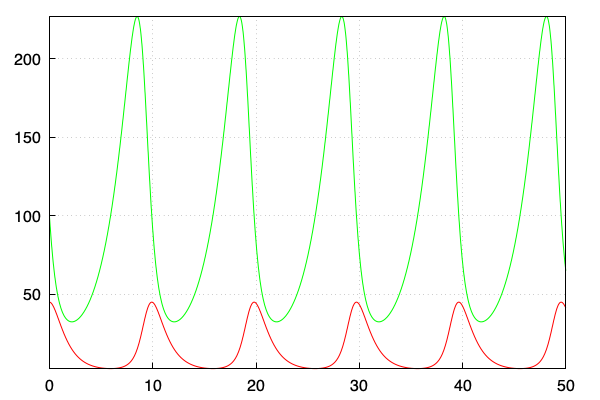
\includegraphics[width=.95\linewidth,height=.80\textheight,keepaspectratio]{lotkavolterra_img/lotkavolterra_1}\mbox{}
\]
%%%%%%%%%%%%%%%
Phasendiagramm (Die y-Achse zeigt die Anzahl der Räuber-, die x-Achse dieAnzahl der Beutetiere):




\noindent
%%%%%%%%%%%%%%%
%%% INPUT:
\begin{minipage}[t]{4em}\color{red}\bf
(\% i12)
\end{minipage}
\begin{minipage}[t]{\textwidth}\color{blue}
wxdraw2d(points(liB, liR));


\end{minipage}
%%% OUTPUT:
\[\displaystyle \tag{\% t12} 
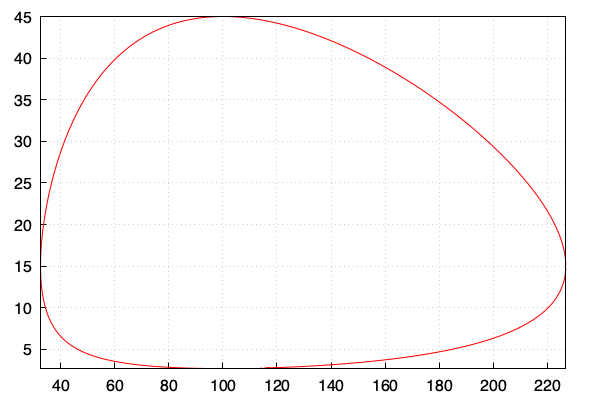
\includegraphics[width=.95\linewidth,height=.80\textheight,keepaspectratio]{lotkavolterra_img/lotkavolterra_2}\mbox{}\]

\[\tag{\% o12} 
\mbox{}
\]
%%%%%%%%%%%%%%%


\noindent
%%%%%%%%%%%%%%%
%%% INPUT:
\begin{minipage}[t]{4em}\color{red}\bf
 \ensuremath{\longrightarrow}  
\end{minipage}
\begin{minipage}[t]{\textwidth}\color{blue}
;


\end{minipage}

\noindent%

\end{document}
